% !TeX program = pdfLaTeX
\documentclass[smallextended]{svjour3}       % onecolumn (second format)
%\documentclass[twocolumn]{svjour3}          % twocolumn
%
\smartqed  % flush right qed marks, e.g. at end of proof
%
\usepackage{amsmath}
\usepackage{graphicx}
\usepackage[utf8]{inputenc}

\usepackage[hyphens]{url} % not crucial - just used below for the URL
\usepackage{hyperref}
\providecommand{\tightlist}{%
  \setlength{\itemsep}{0pt}\setlength{\parskip}{0pt}}

%
% \usepackage{mathptmx}      % use Times fonts if available on your TeX system
%
% insert here the call for the packages your document requires
%\usepackage{latexsym}
% etc.
%
% please place your own definitions here and don't use \def but
% \newcommand{}{}
%
% Insert the name of "your journal" with
% \journalname{myjournal}
%

%% load any required packages here



% Pandoc citation processing


\begin{document}

\title{Perdiz arrow points from Caddo burial contexts aid in defining
discrete behavioral regions \thanks{Components of the analytical
workflow were developed and funded by a Preservation Technology and
Training grant (P14AP00138) to RZS from the National Center for
Preservation Technology and Training, as well as grants to RZS from the
Caddo Nation of Oklahoma, National Forests and Grasslands in Texas
(15-PA-11081300-033) and the United States Forest Service
(20-PA-11081300-074).} }


    \titlerunning{Perdiz arrow points from Caddo burial contexts}

\author{  Robert Z. Selden 1 \and  John E. Dockall 2 \and  }

    \authorrunning{ Selden and Dockall }

\institute{
        Robert Z. Selden 1 \at
     Heritage Research Center and Department of Biology, Stephen F.
Austin State University; and Cultural Heritage Department, Jean Monnet
University \\
     \email{\href{mailto:zselden@sfasu.edu}{\nolinkurl{zselden@sfasu.edu}}}  %  \\
%             \emph{Present address:} of F. Author  %  if needed
    \and
        John E. Dockall 2 \at
     Cox\textbar McClain Environmental Consultants, Inc. \\
     \email{\href{mailto:johnd@coxmcclain.com}{\nolinkurl{johnd@coxmcclain.com}}}  %  \\
%             \emph{Present address:} of F. Author  %  if needed
    \and
    }

\date{Received: date / Accepted: date}
% The correct dates will be entered by the editor


\maketitle

\begin{abstract}
Recent research in the ancestral Caddo area has yielded evidence for
distinct \emph{behavioral regions}, across which material culture from
Caddo burials---Hickory Engraved and Smithport Plain bottles as well as
Gahagan bifaces---has been found to express significant morphological
differences. This inquiry assesses whether Perdiz arrow points from
Caddo burials, assumed to reflect design intent, may differ across the
same geography, and extend the pattern of shape differences to a third
category of Caddo material culture. Perdiz arrow points collected from
the geographies of the northern and southern Caddo \emph{behavioral
regions} defined in a recent social network analysis were employed to
test the hypothesis that morphological attributes differ, and are
predictable, between the two communities. Results indicate significant
between-community differences in maximum length, width, stem length, and
stem width, but not thickness. Using the same traditional metrics
combined with the tools of machine learning, a predictive
model---support vector machine---was designed to assess the degree to
which community differences could be predicted, achieving a receiver
operator curve score of 97 percent, and an accuracy score of 94 percent.
The subsequent geometric morphometric analysis identified significant
differences in Perdiz arrow point shape, size, and allometry, coupled
with significant results for modularity and morphological integration.
These findings bolster recent arguments that established two discrete
\emph{behavioral regions} in the ancestral Caddo area, which are defined
on the basis of discernible morphological differences across three
categories of Caddo material culture.
\\
\keywords{
        American Southeast \and
        Caddo \and
        Texas \and
        archaeoinformatics \and
        computational archaeology \and
        machine learning \and
        museum studies \and
        digital humanities \and
        STEM \and
    }


\end{abstract}


\def\spacingset#1{\renewcommand{\baselinestretch}%
{#1}\small\normalsize} \spacingset{1}


\hypertarget{intro}{%
\section{Introduction}\label{intro}}

Perdiz arrow points generally follow two distinct manufacturing
trajectories; one that enlists flakes, and the other, blade flakes
\cite{RN8999,RN9361,RN9000,RN9364}. Lithic tool stone in the Caddo area
of northeast Texas is relatively sparse, consists primarily of chert,
quartzite, and silicified wood characteristic of the local geological
formations, which may contribute to local variation in both morphology
and size \cite{RN9364,RN439}. It has been demonstrated elsewhere that
Perdiz arrow points from northeast Texas vary significantly by time, raw
material, and burial context \cite{RN9364}. In outline, Perdiz arrow
points possess a:

\begin{quote}
{[}t{]}riangular blade with edges usually quite straight but sometimes
slightly convex or concave. Shoulders sometimes at right angles to stem
but usually well barbed. Stem contracted, often quite sharp at base, but
may be somewhat rounded. Occasionally, specimen may be worked on one
face only or mainly on one face \ldots{} {[}w{]}orkmanship generally
good, sometimes exceedingly fine with minutely serrated blade edges
\cite[504]{RN5769}.
\end{quote}

A social network analysis of Historic Caddo (post-CE 1680) sites in
northeast Texas demonstrated two spatially distinct \emph{behavioral
regions} \cite{RN8031} (Fig. 1). The network analysis was limited to
Historic Caddo types; however, Formative Early Caddo (CE 800 -- 1200)
Gahagan bifaces and Caddo bottle types have been found to express
significantly different morphologies between the same two areas
\cite{RN8074,RN7927,RN8370,RN8312}, extending the temporal range of the
shape boundary. Gahagan bifaces from the ancestral Caddo area also
differ significantly in shape, size, and form from those recovered at
central Texas sites \cite{RN8322}, suggestive of a second shape boundary
between the Caddo region and central Texas.

\begin{figure}
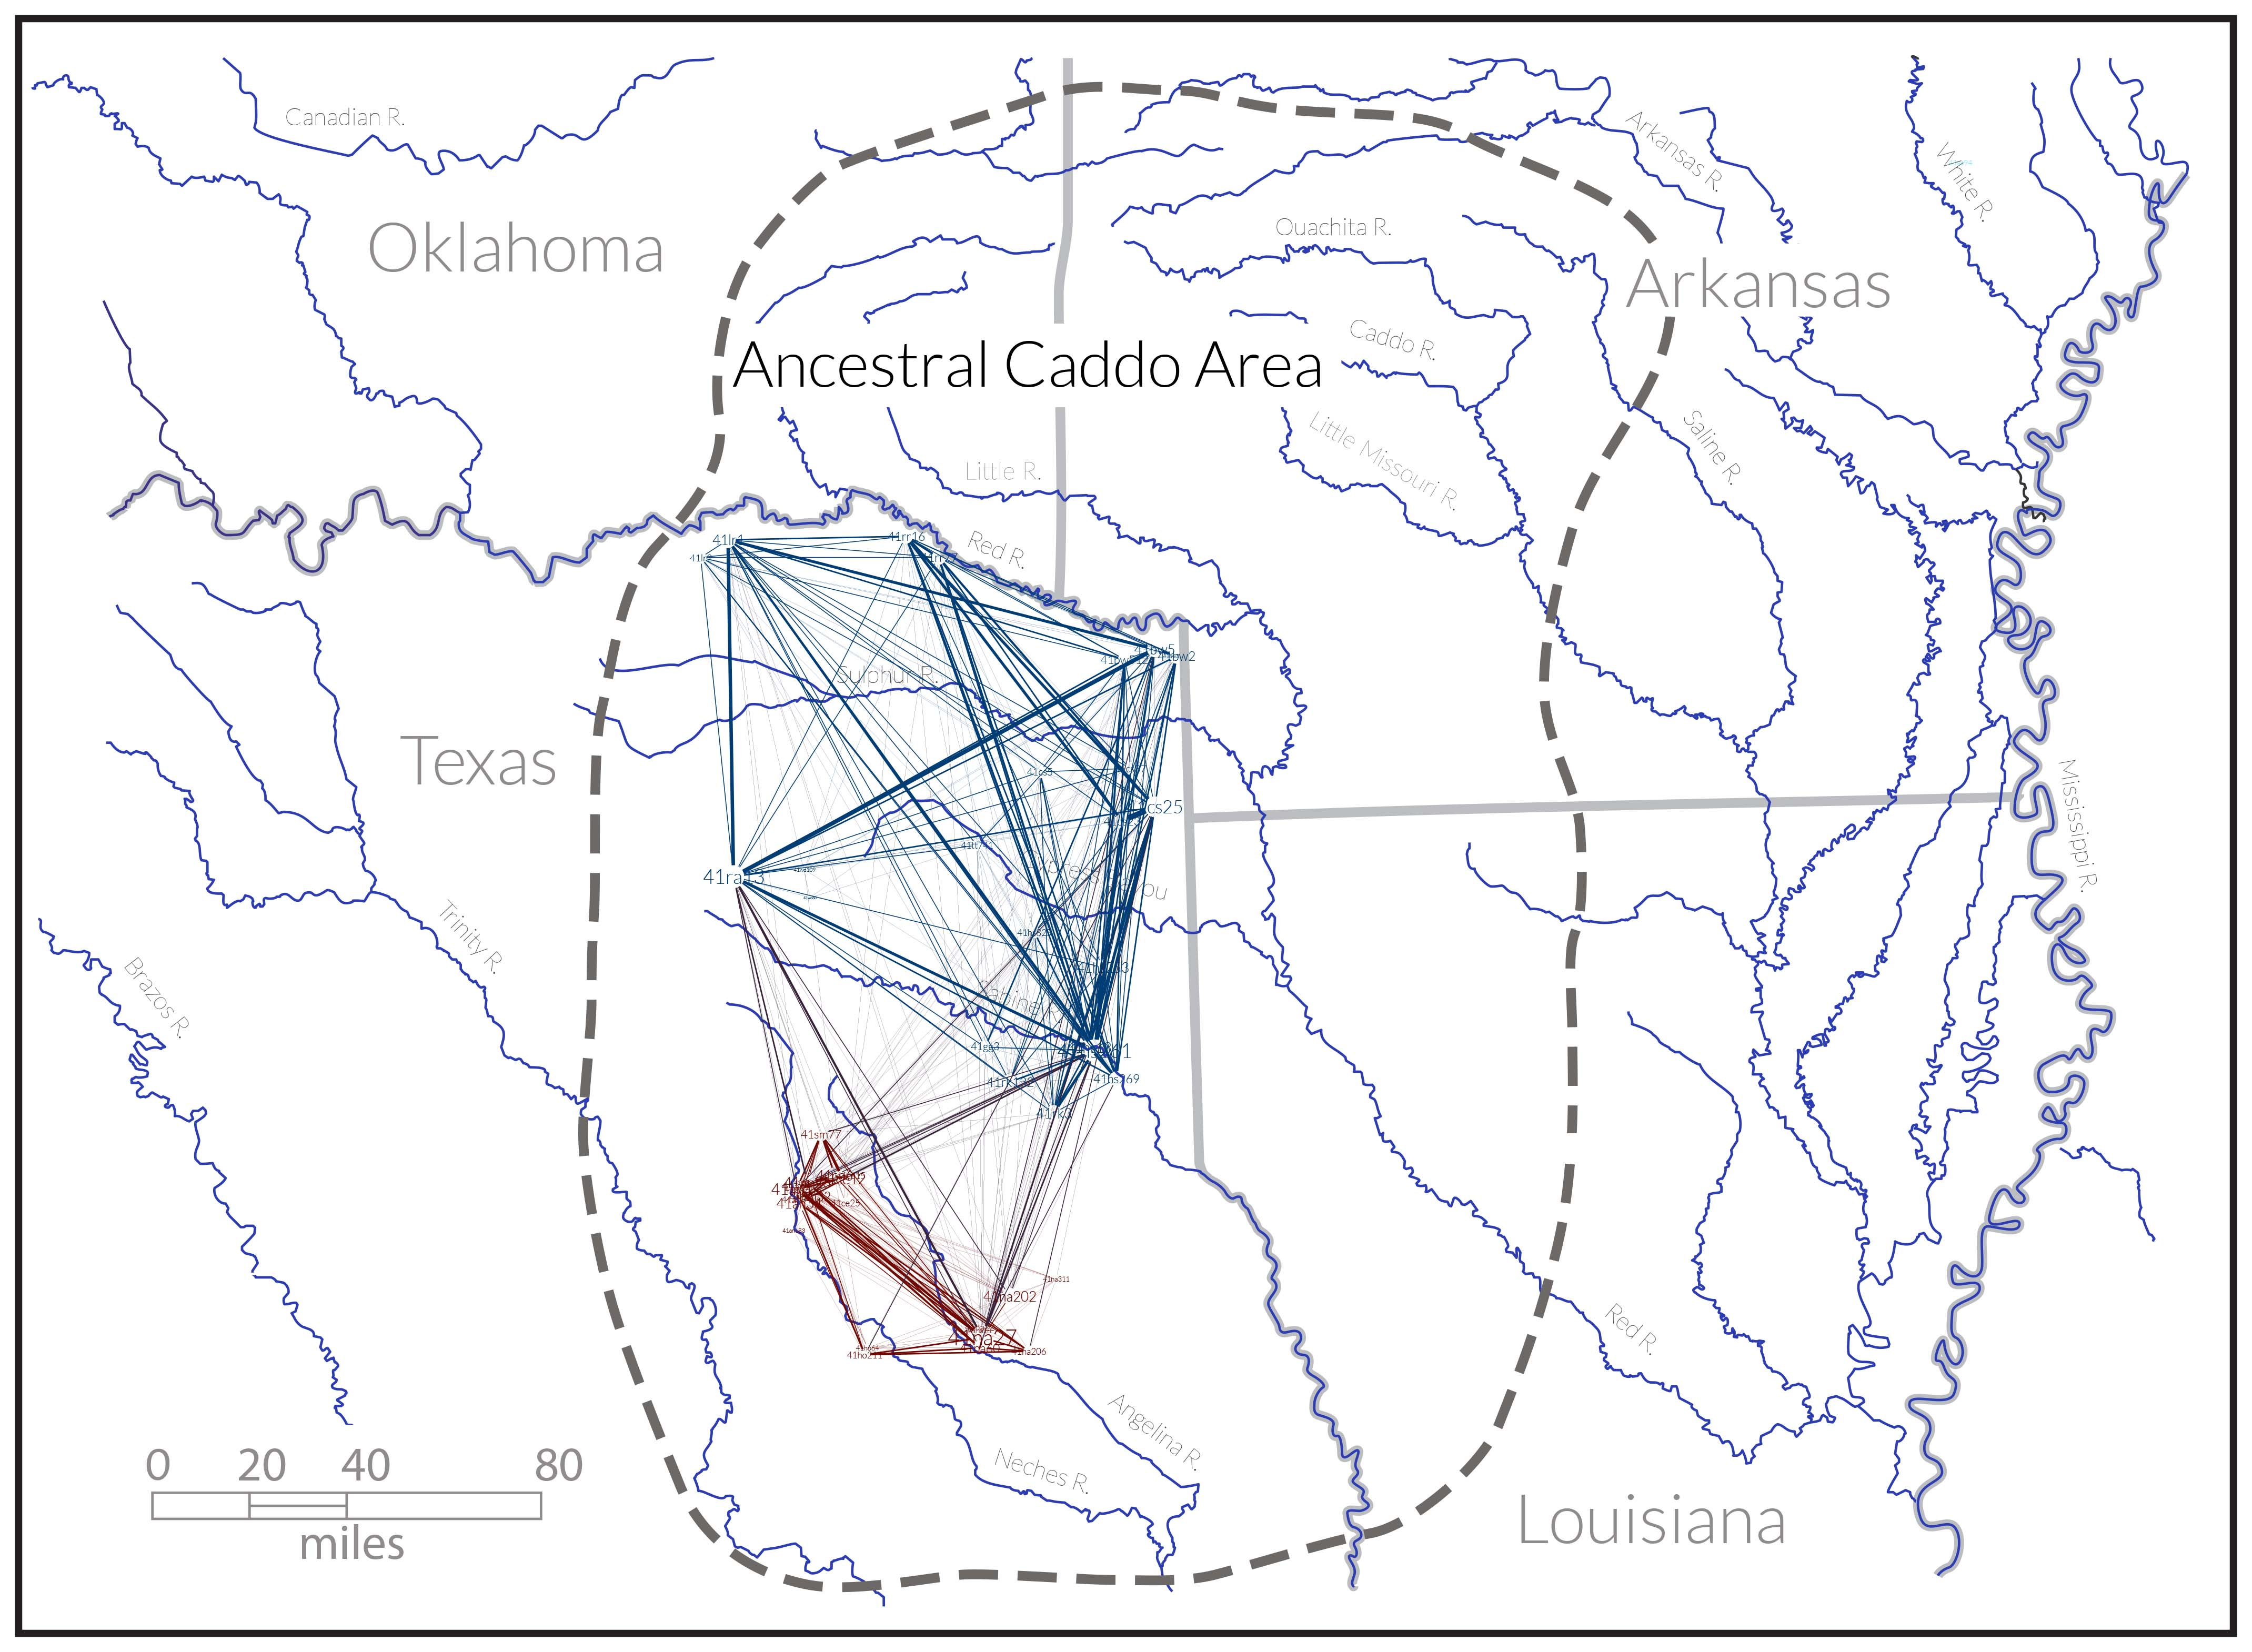
\includegraphics[width=1\linewidth]{ms-figs/figure1} \caption{Historic Caddo network generated using ceramic and lithic types, which include Perdiz arrow points (DOI 10.17605/OSF.IO/WD2ZT), illustrating the two (north [blue] and south [red]) Caddo behavioral regions. The regions were identified using a modularity statistic to identify those nodes more densely connected to one another than to the rest of the network .}\label{fig:fig1}
\end{figure}

The goal of this exploratory endeavor was to assess whether traditional
metrics collected for Perdiz arrow points support the \emph{shape
boundary} posited in recent social network and geometric morphometric
analyses, to determine whether linear metrics might be useful predictors
of regional membership, and---if so---to identify those morphological
features that articulate with each \emph{behavioral region} using
geometric morphometrics. It is assumed that complete Perdiz arrow points
included as offerings in Caddo burials represent the design intent of
the maker. Should the analysis yield significant results, it would
bolster the argument for at least two discrete Caddo \emph{behavioral
regions}; each empirically defined by discernible morphological
differences across three discrete categories of Caddo material culture.

\hypertarget{caddo-behavioral-regions}{%
\subsection{\texorpdfstring{\emph{Caddo behavioral
regions}}{Caddo behavioral regions}}\label{caddo-behavioral-regions}}

In a June 18, 1937 Works Progress Administration interview with Lillian
Cassaway, Sadie Bedoka---a Caddo-Delaware woman raised with the
Caddo---stated that:

\begin{quote}
Each {[}Caddo{]} clan had its own shape to make its pottery. One clan
never thought of making anything the same pattern of another clan.
\emph{You could tell who made the pottery by the shape}
\cite[395]{RN9357x}.
\end{quote}

General differences in Caddo ceramic forms have been noted elsewhere
\cite{RN5650,RN7129,RN7162}; however, the study of the Clarence H. Webb
collection was the first to illustrate a significant north-south
geographic shape difference among Hickory Engraved and Smithport Plain
Caddo bottle types \cite{RN8370}. That preliminary observation was later
confirmed using more robust samples of Hickory Engraved and Smithport
Plain bottles \cite{RN8074,RN7927}, then expanded to include a greater
variety of Caddo bottle types across a larger spatial extent
\cite{RN8312}.

The co-presence of diagnostic artifact and attribute types have been
used to define the Caddo phases and periods that serve as a heuristic
tool to aid archaeologists in explaining the local cultural landscape.
The Historic Caddo network expands those efforts, augmenting the
previously defined phases and periods, and emphasizing the dynamic and
manifold relational connections that transcend the currently-defined
categories \cite{RN8031}. This was achieved by enlisting a multi-scalar
methodological approach \cite{RN5644,RN8039}, where the northern and
southern communities were parsed into constituent groups using
diagnostic types paired with a modularity statistic
\cite{RN8051,RN8024}. A number of the constituent groups identified by
the networks were found to articulate with known Caddo polities, while
others were not \cite{RN8031}.

A subsequent analysis of Gahagan bifaces confirmed that a second
category of Caddo material culture expressed significant morphological
differences across the same geography as the Hickory Engraved and
Smithport Plain bottles \cite{RN8158}. The morphology of Gahagan bifaces
from sites in central Texas was later found to differ significantly when
compared with those recovered from the Caddo region \cite{RN8322}. That
Gahagan bifaces were found to differ across two spatial boundaries was
noteworthy, particularly since it has regularly been assumed that these
large bifaces were manufactured in central Texas and arrived in the
ancestral Caddo area as products of trade and/or exchange
\cite{RN8322,RN8158}. Further, that Gahagan bifaces were found to differ
across the same geography as those communities posited in the Historic
Caddo network analysis suggested that the temporal range of the shape
boundary might extend to the Formative/Early Caddo period (CE 800 -
1250); a hypothesis that was later confirmed in a more comprehensive
analysis of Caddo bottles \cite{RN8312}.

\hypertarget{methods-and-results}{%
\section{Methods and results}\label{methods-and-results}}

Sixty seven intact Perdiz arrow points from Caddo burials in Camp,
Nacogdoches, and Shelby counties were used for this study
(\href{https://seldenlab.github.io/perdiz3/}{supplementary materials}).
A standard suite of linear metrics was collected for each specimen,
including maximum length, width, thickness, stem length, and stem width.
Following collection, data were imported to R
(\href{https://seldenlab.github.io/perdiz3/}{supplementary materials}),
where boxplots were produced, along with a Principal Components Analysis
(PCA) followed by analyses of variance (ANOVA) to test whether the
morphology of Perdiz arrow points differs across the shape boundary
(Fig.2).

Boxplots illustrate the distribution and mean for each of the five
variables (Fig. 2a-e), and the PCA (Fig. 2f) illustrates over 92 percent
of the variation in the sample among PC1 (84.65 percent) and PC2 (11.71
percent). The ANOVAs demonstrate significant differences in Perdiz arrow
point morphology among four of the five variables (maximum length,
width, stem length, and stem width)
(\href{https://seldenlab.github.io/perdiz3/}{supplementary materials}).
Maximum thickness does not differ significantly between the northern and
southern communities, which led to the decision to conduct the
subsequent geometric morphometric analysis as a two dimensional, rather
than a three-dimensional, study
(\href{https://seldenlab.github.io/perdiz3/}{supplementary materials}).

\begin{figure}
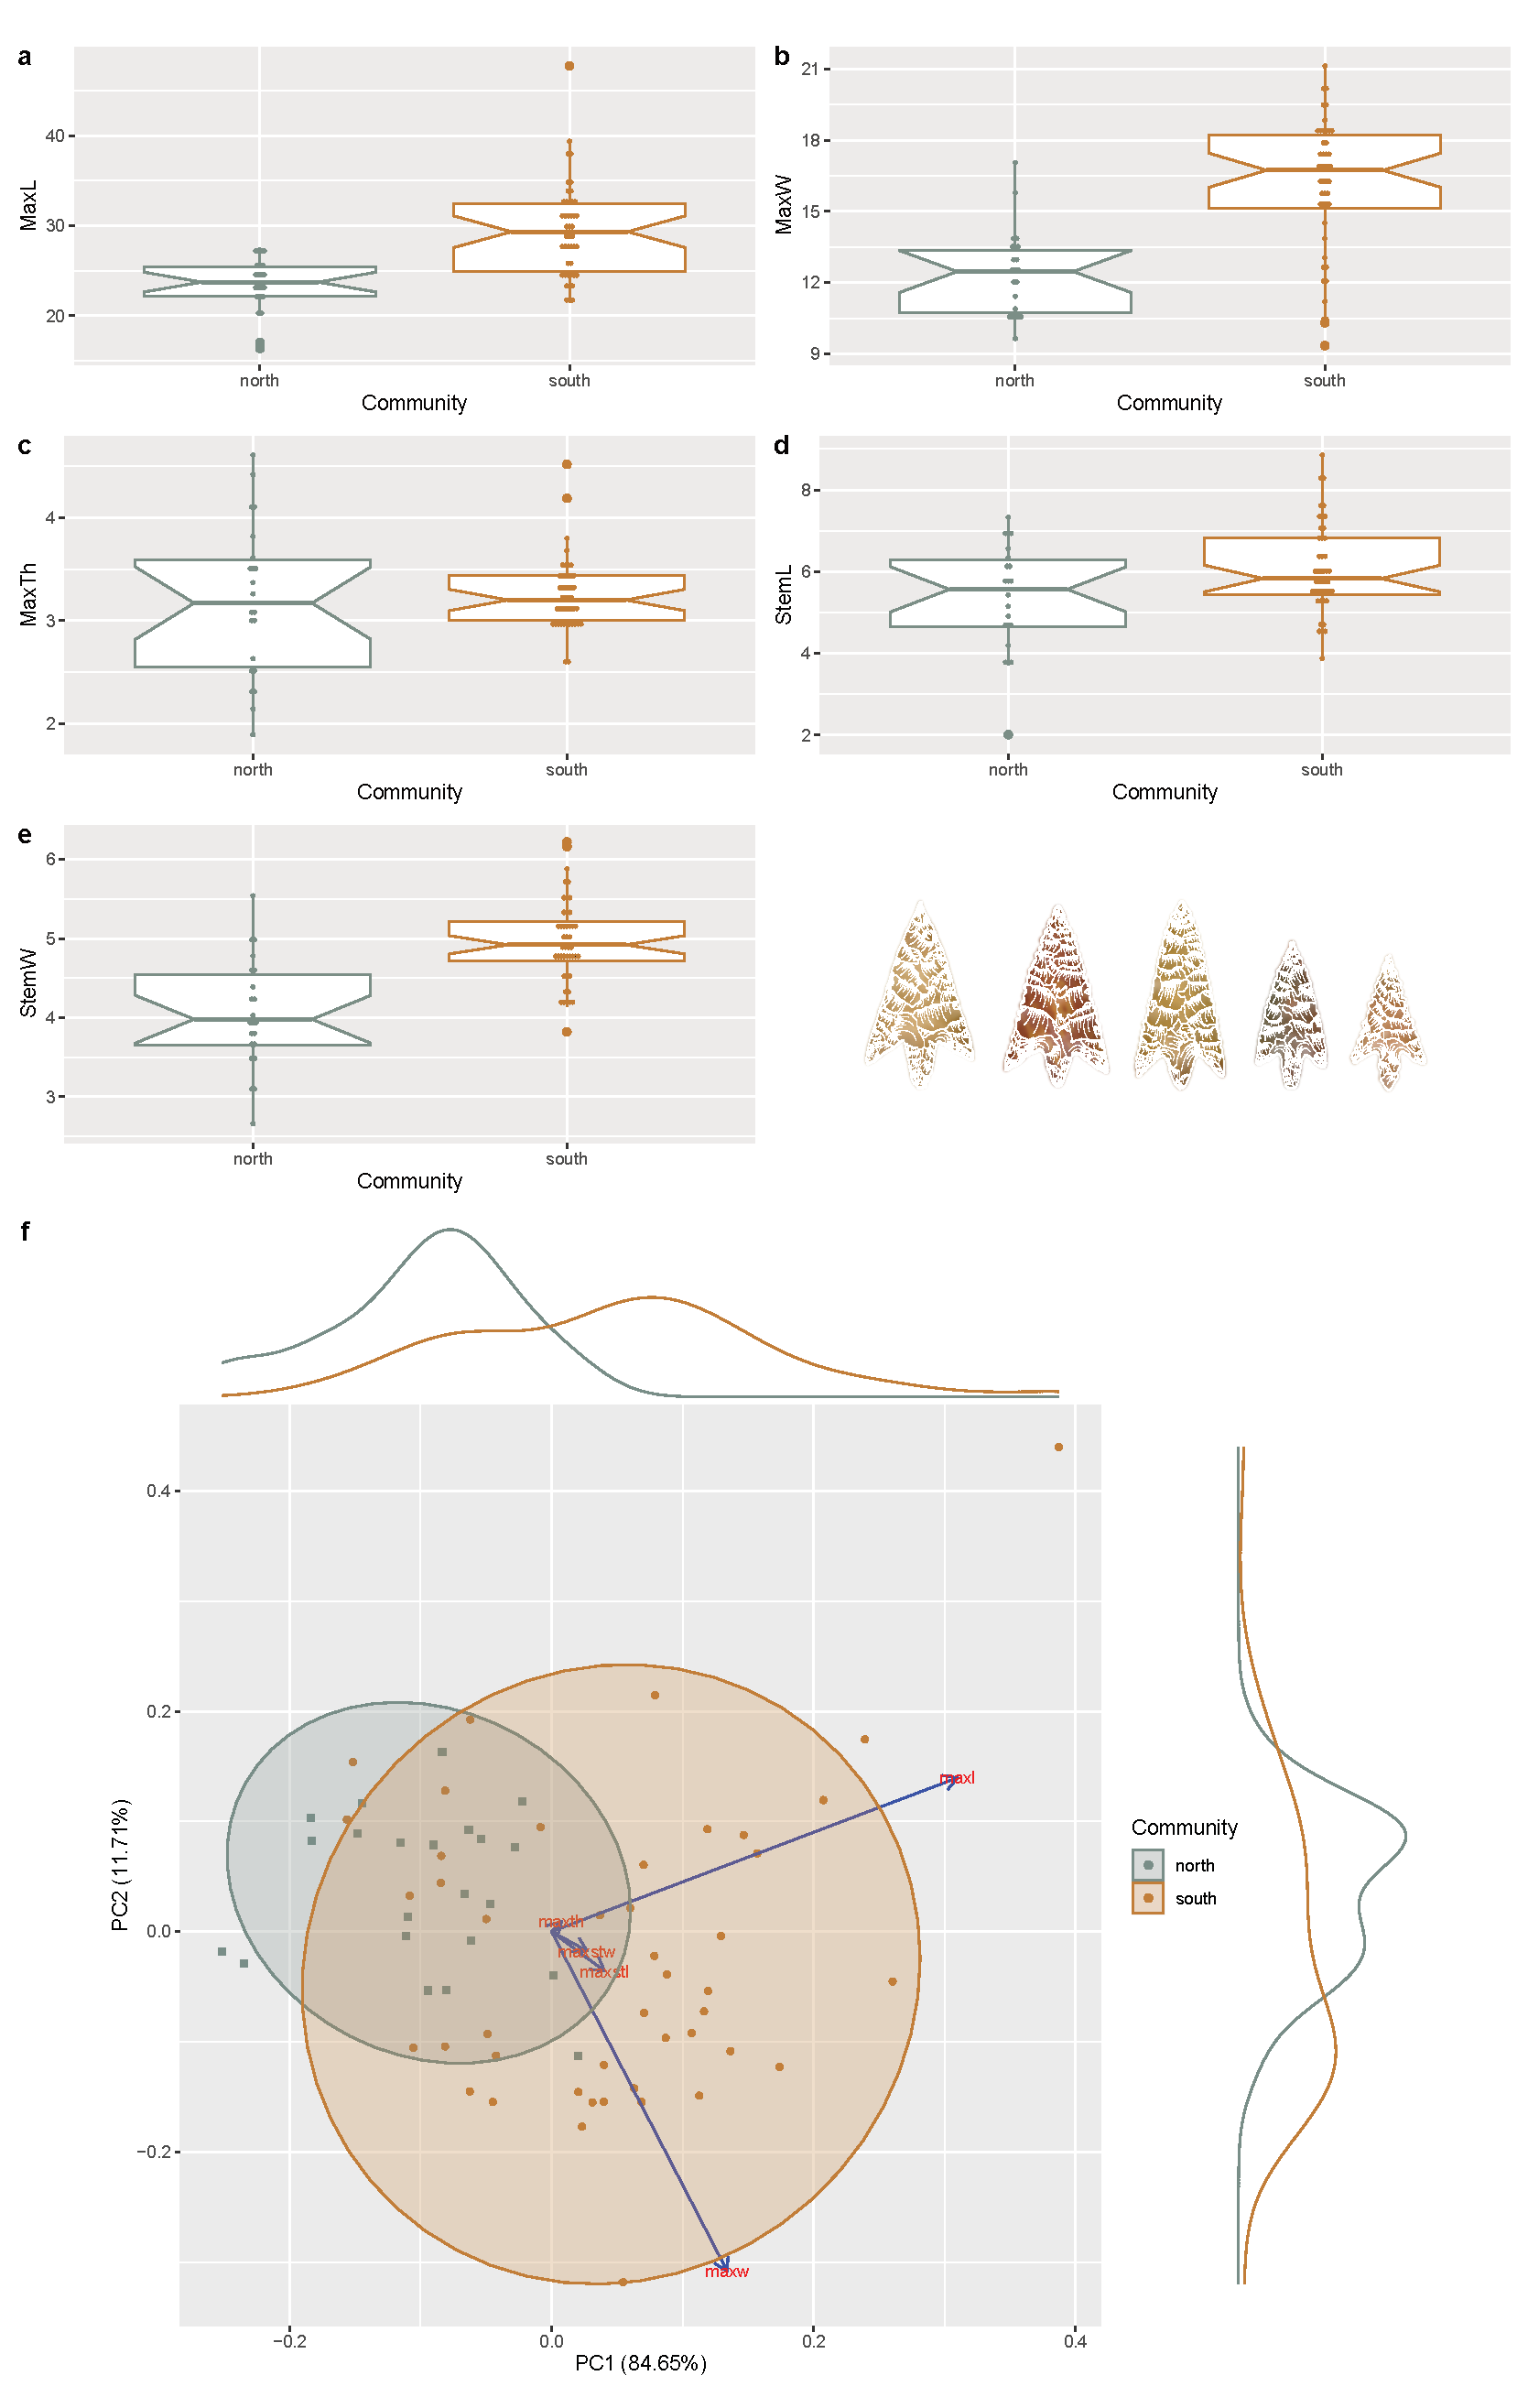
\includegraphics[width=0.95\linewidth]{ms-figs/figure2} \caption{Boxplots for a, maximum length; b, maximum width; c, maximum thickness; d, stem length; e, stem width, and f, PCA for linear metrics associated with the Perdiz arrow points. Additional information related to the analysis, including data and code needed to reproduce these results, can be found in the supplemental materials at https://seldenlab.github.io/perdiz3/.}\label{fig:fig2}
\end{figure}

\hypertarget{predictive-model}{%
\subsection{\texorpdfstring{\emph{Predictive
model}}{Predictive model}}\label{predictive-model}}

For the support vector machine, linear data were imported to Python
(\href{https://seldenlab.github.io/perdiz3/}{supplementary materials}),
where they were split into training (75 percent) and testing (25
percent) subsets. A standard scaler was used to decrease the sensitivity
of the algorithm to outliers by standardizing features, and a nested
cross validation of the training set was used to achieve unbiased
estimates of model performance, resulting in a mean cross validation
score of 86 percent
(\href{https://seldenlab.github.io/perdiz3/}{supplementary materials}).
The model was subsequently fit on the training set, yielding a receiver
operator curve score of 97 percent, and an accuracy score of 94 percent
(\href{https://seldenlab.github.io/perdiz3/}{supplementary materials}).

\hypertarget{geometric-morphometrics}{%
\subsection{\texorpdfstring{\emph{Geometric
morphometrics}}{Geometric morphometrics}}\label{geometric-morphometrics}}

Each of the arrow points was imaged using a flatbed scanner (HP Scanjet
G4050) at 600 dpi. The landmarking protocol developed for this study
(\href{https://seldenlab.github.io/perdiz3/}{supplementary materials})
includes six landmarks and 24 equidistant semilandmarks to characterize
Perdiz arrow point shape, and were applied using the
\texttt{StereoMorph} package in R \cite{RN8973}. The characteristic
points and tangents used in the landmarking protocol were inspired by
the work of Birkhoff \cite{RN5700}.

Landmark data were aligned to a global coordinate system
\cite{RN8102,RN8587,RN8384}, achieved through generalized Procrustes
superimposition \cite{RN8525} performed in R 4.1.1 \cite{RN8584} using
the \texttt{geomorph} package v4.0.0 \cite{RN8565}. Procrustes
superimposition translates, scales, and rotates the coordinate data
allowing for comparisons among objects \cite{RN5698,RN8525}. The
\texttt{geomorph} package uses a partial Procrustes superimposition that
projects the aligned specimens into tangent space subsequent to
alignment in preparation for the use of multivariate methods that assume
linear space \cite{RN8511,RN8384} (Fig.3).

\begin{figure}
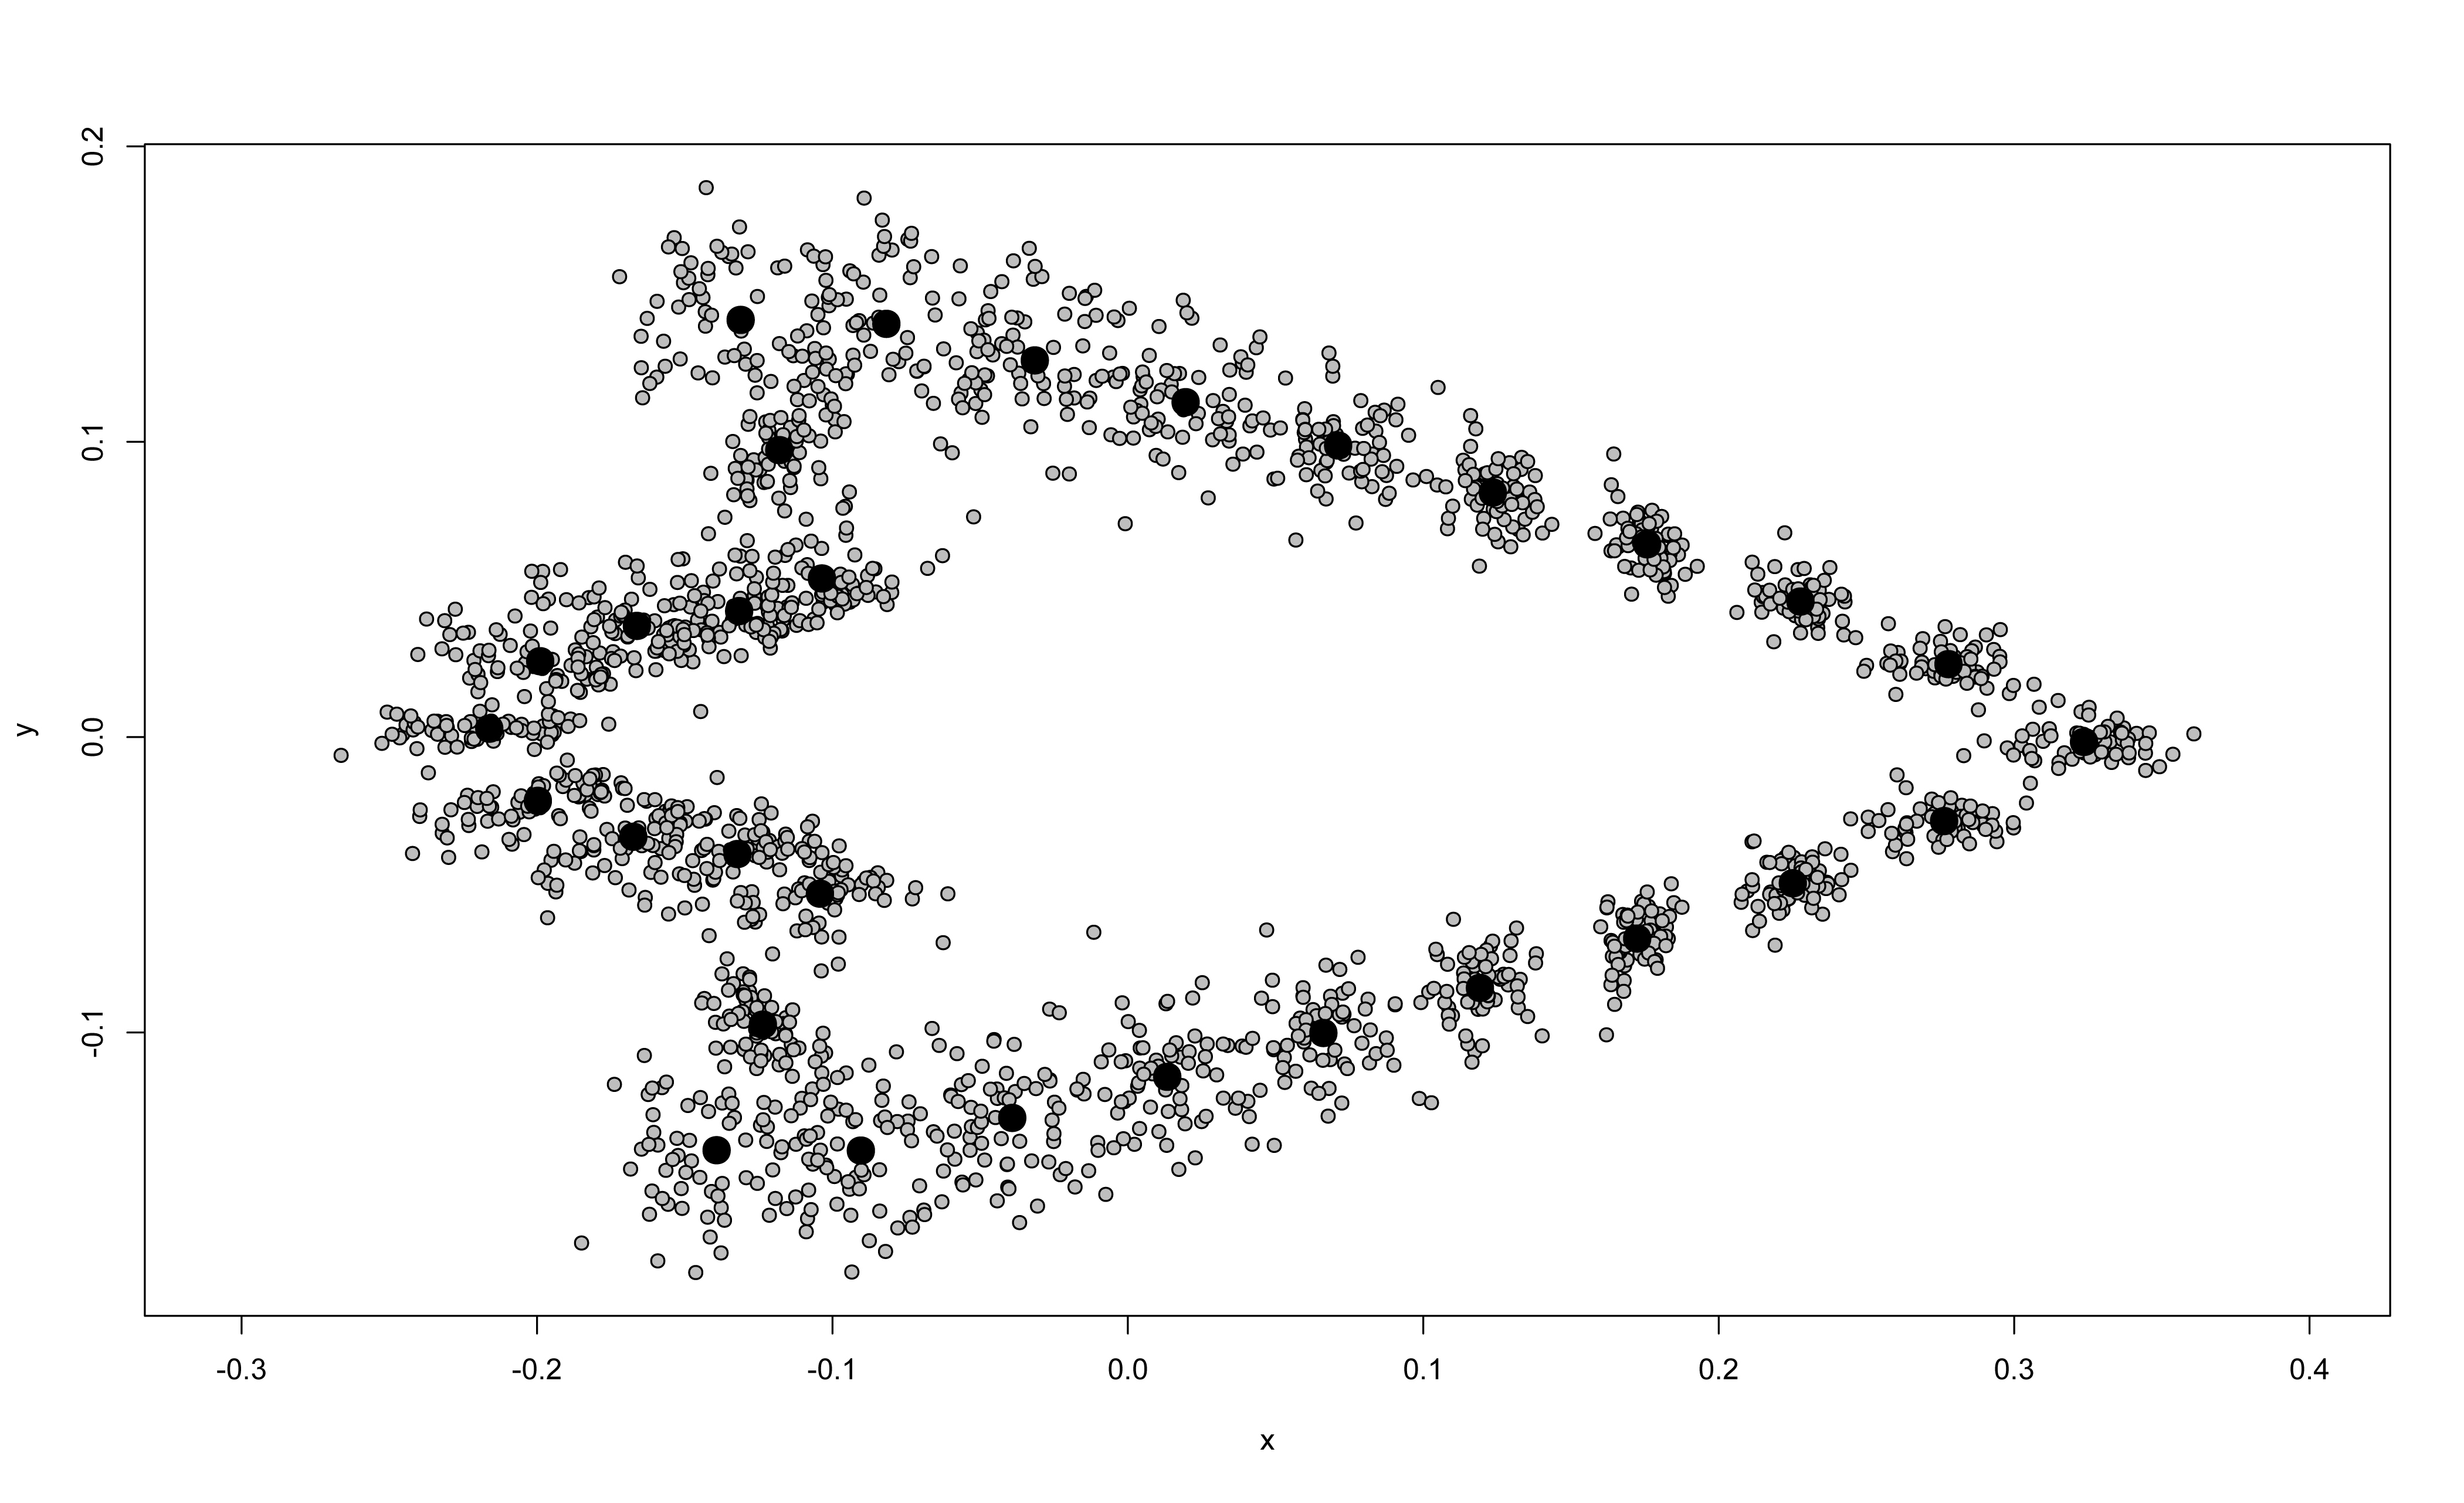
\includegraphics[width=1\linewidth]{ms-figs/figure3} \caption{Results of generalized Procrustes analysis, illustrating mean shape (black) and all specimens in the sample (gray). Additional information related to the GPA, including those data and code needed to reproduce these results, can be found in the supplemental materials at https://seldenlab.github.io/perdiz3/.}\label{fig:fig3}
\end{figure}

Principal components analysis \cite{RN8576} was used to visualize shape
variation among the arrow points (Fig. 4). The shape changes described
by each principal axis are commonly visualized using thin-plate spline
warping of a reference image or 3D mesh \cite{RN8555,RN8553}. A residual
randomization permutation procedure (RRPP; n = 10,000 permutations) was
used for all Procrustes ANOVAs \cite{RN8579,RN8334}, which has higher
statistical power and a greater ability to identify patterns in the data
should they be present \cite{RN6995}. To assess whether shape changes
with size (allometry), and differs by group (region), Procrustes ANOVAs
\cite{RN7046} were also run that enlist effect-sizes (z-scores) computed
as standard deviates of the generated sampling distributions
\cite{RN8477}. Procrustes variance was used to discriminate between
regions and compare the amount of shape variation (morphological
disparity) \cite{RN5703}, estimated as the Procrustes variance using
residuals of linear model fit \cite{RN8314}. A pairwise comparison of
morphological integration was used to test the strength of integration
between blade and basal morphology using a z-score \cite{RN8340}.

\begin{figure}
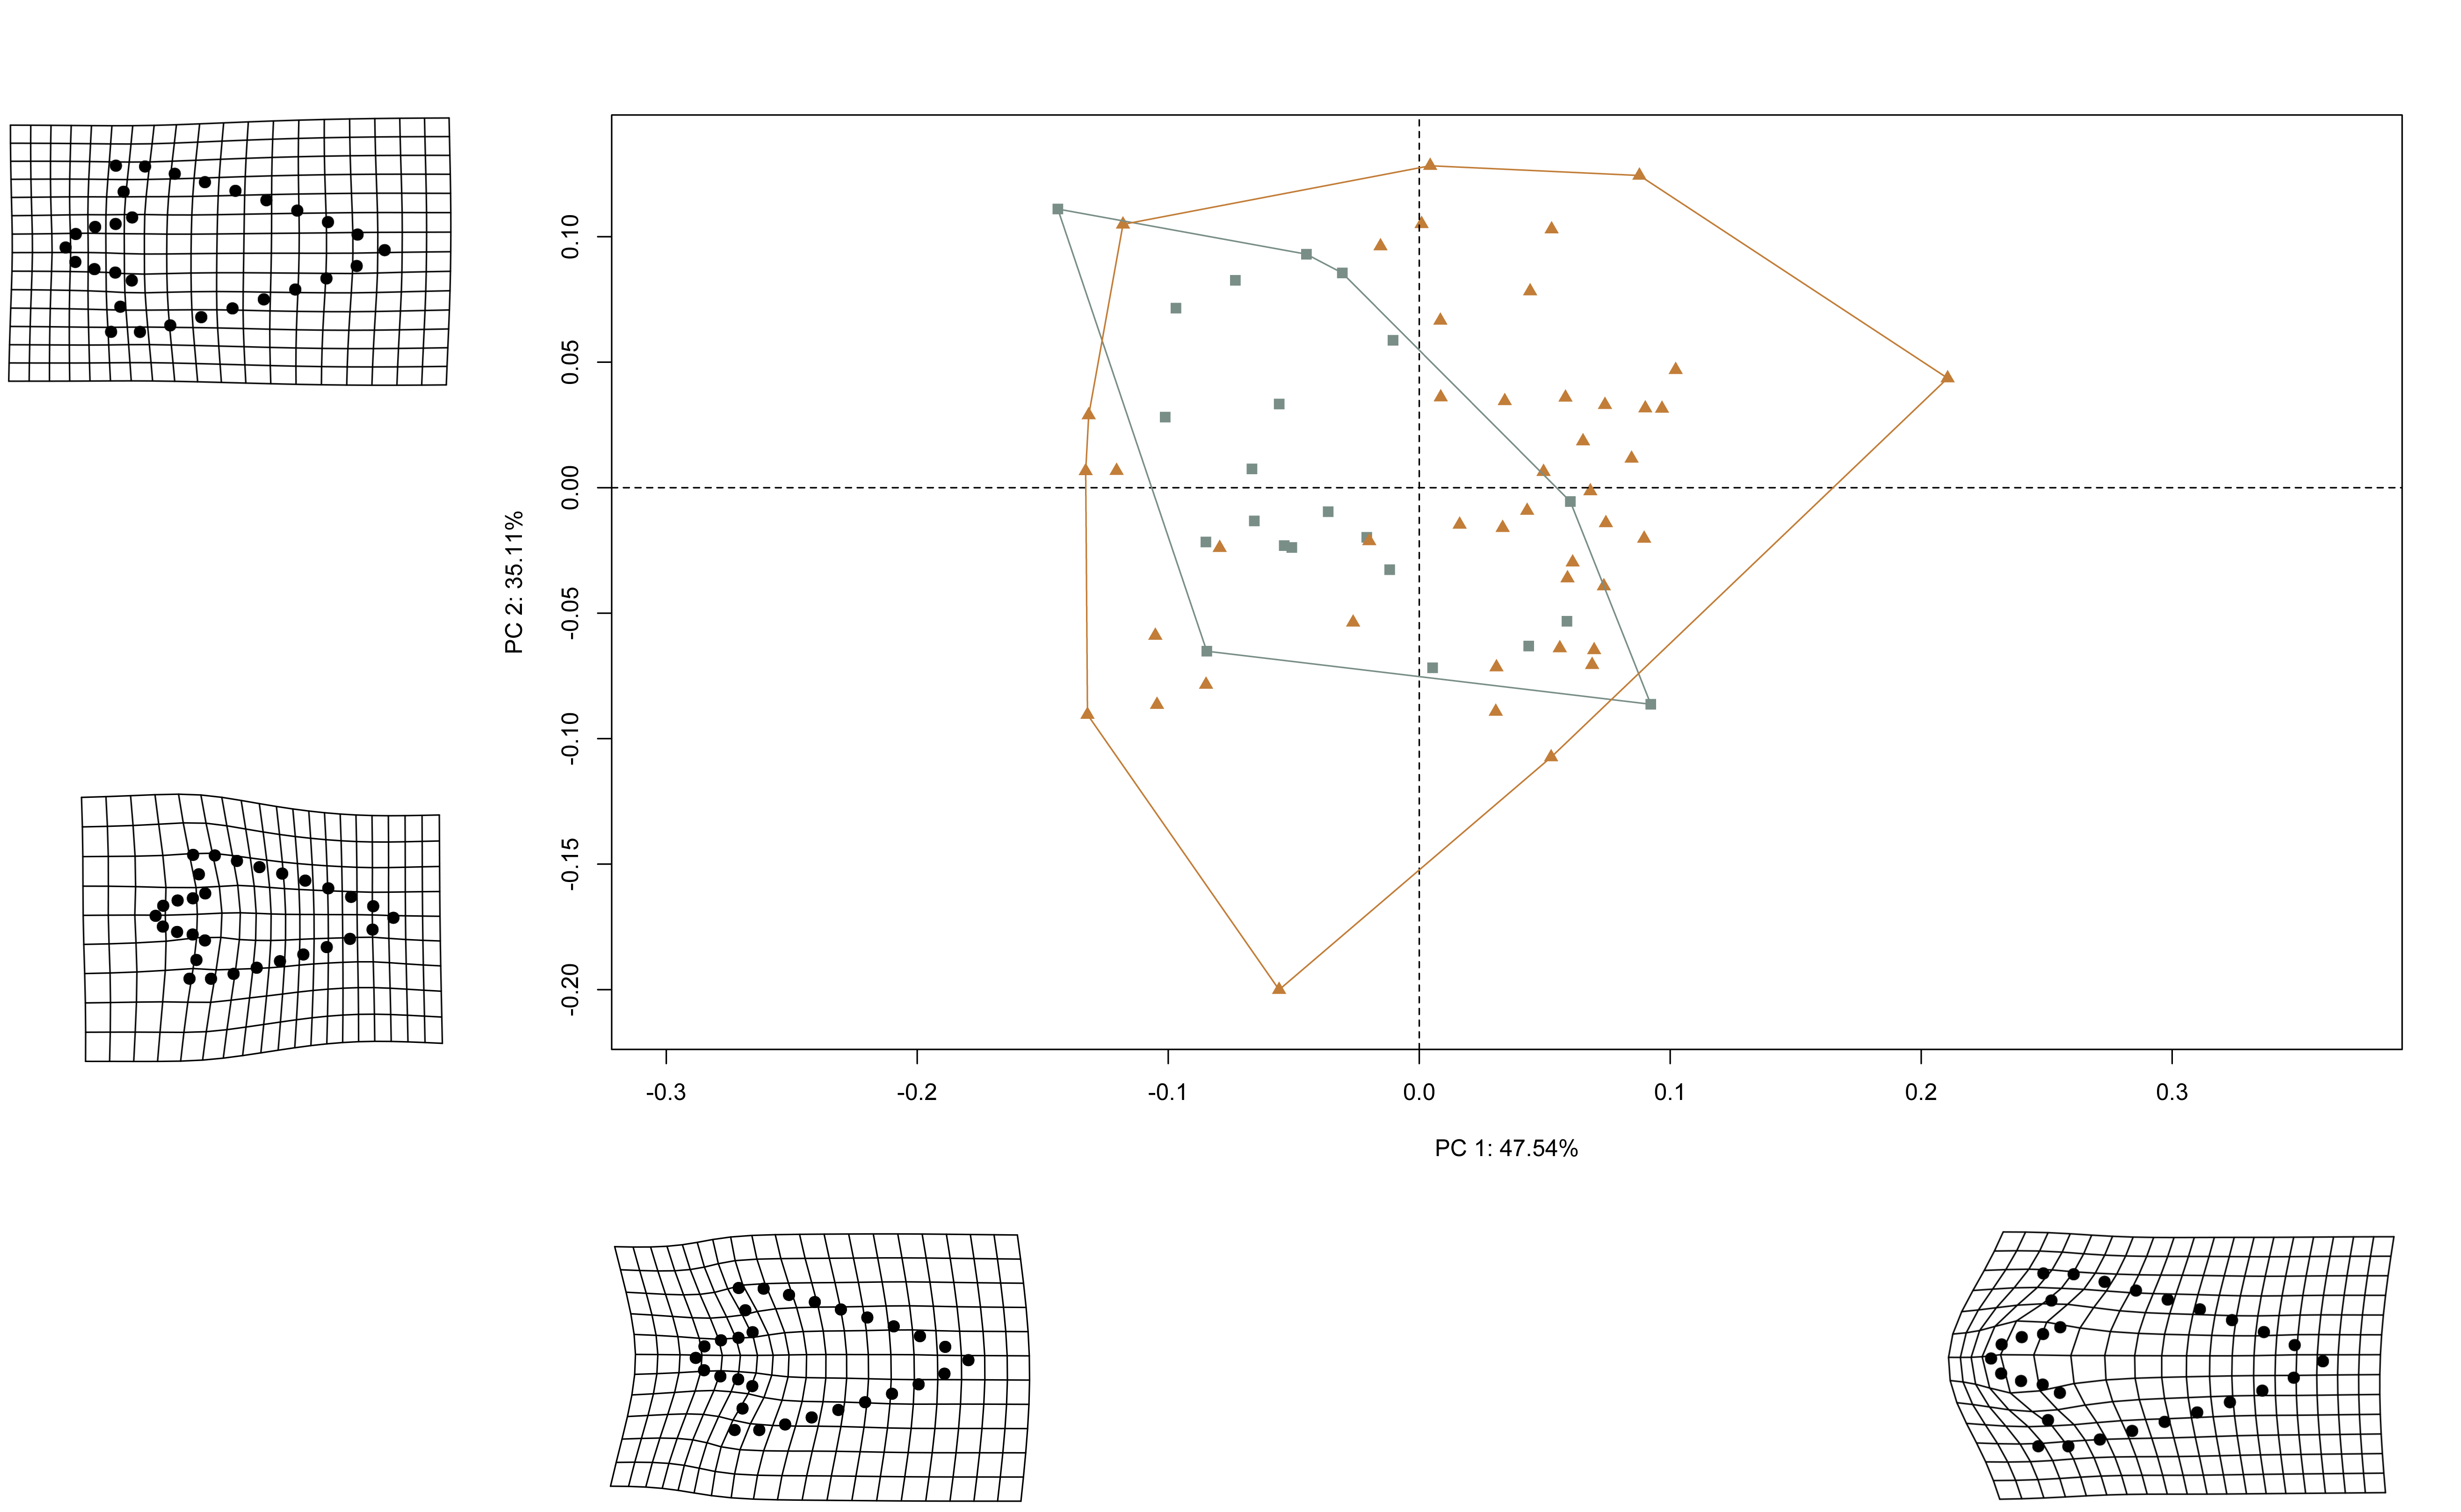
\includegraphics[width=1\linewidth]{ms-figs/figure4} \caption{Principal components analysis plot (PC1/PC2) for Perdiz arrow points by behavioral region/community (top; gray squares, north; orange triangles, south), and results of modularity (bottom left) and blade/base morphological integration (bottom right) analyses. Additional information related to the PCA, including the full listing of results and those data and code needed to reproduce these results, can be found in the supplemental materials at https://seldenlab.github.io/perdiz3/.}\label{fig:fig4}
\end{figure}

A Procrustes ANOVA was used to test whether a significant difference
exists in Perdiz arrow point (centroid) size, and results indicate a
significant difference (RRPP = 10,000; Rsq = 0.30681; Pr(\textgreater F)
= 1e-04). A second Procrustes ANOVA was used to test whether a
significant difference exists in arrow point shape by region (northern
vs.~southern communities), and results indicate a significant difference
(RRPP = 10,000; Rsq = 0.0536; Pr(\textgreater F) = 0.0161). A comparison
of mean consensus configurations was used to characterize intraspecific
shape variation of Perdiz arrow points from the northern and southern
\emph{behavioral regions}. Differential morphology occurs in the basal
area, where the angle between the shoulder and base is more acute, with
a base that is generally shorter and narrower in the southern
\emph{behavioral region} than it is to the north (Fig. 5).

\begin{figure}
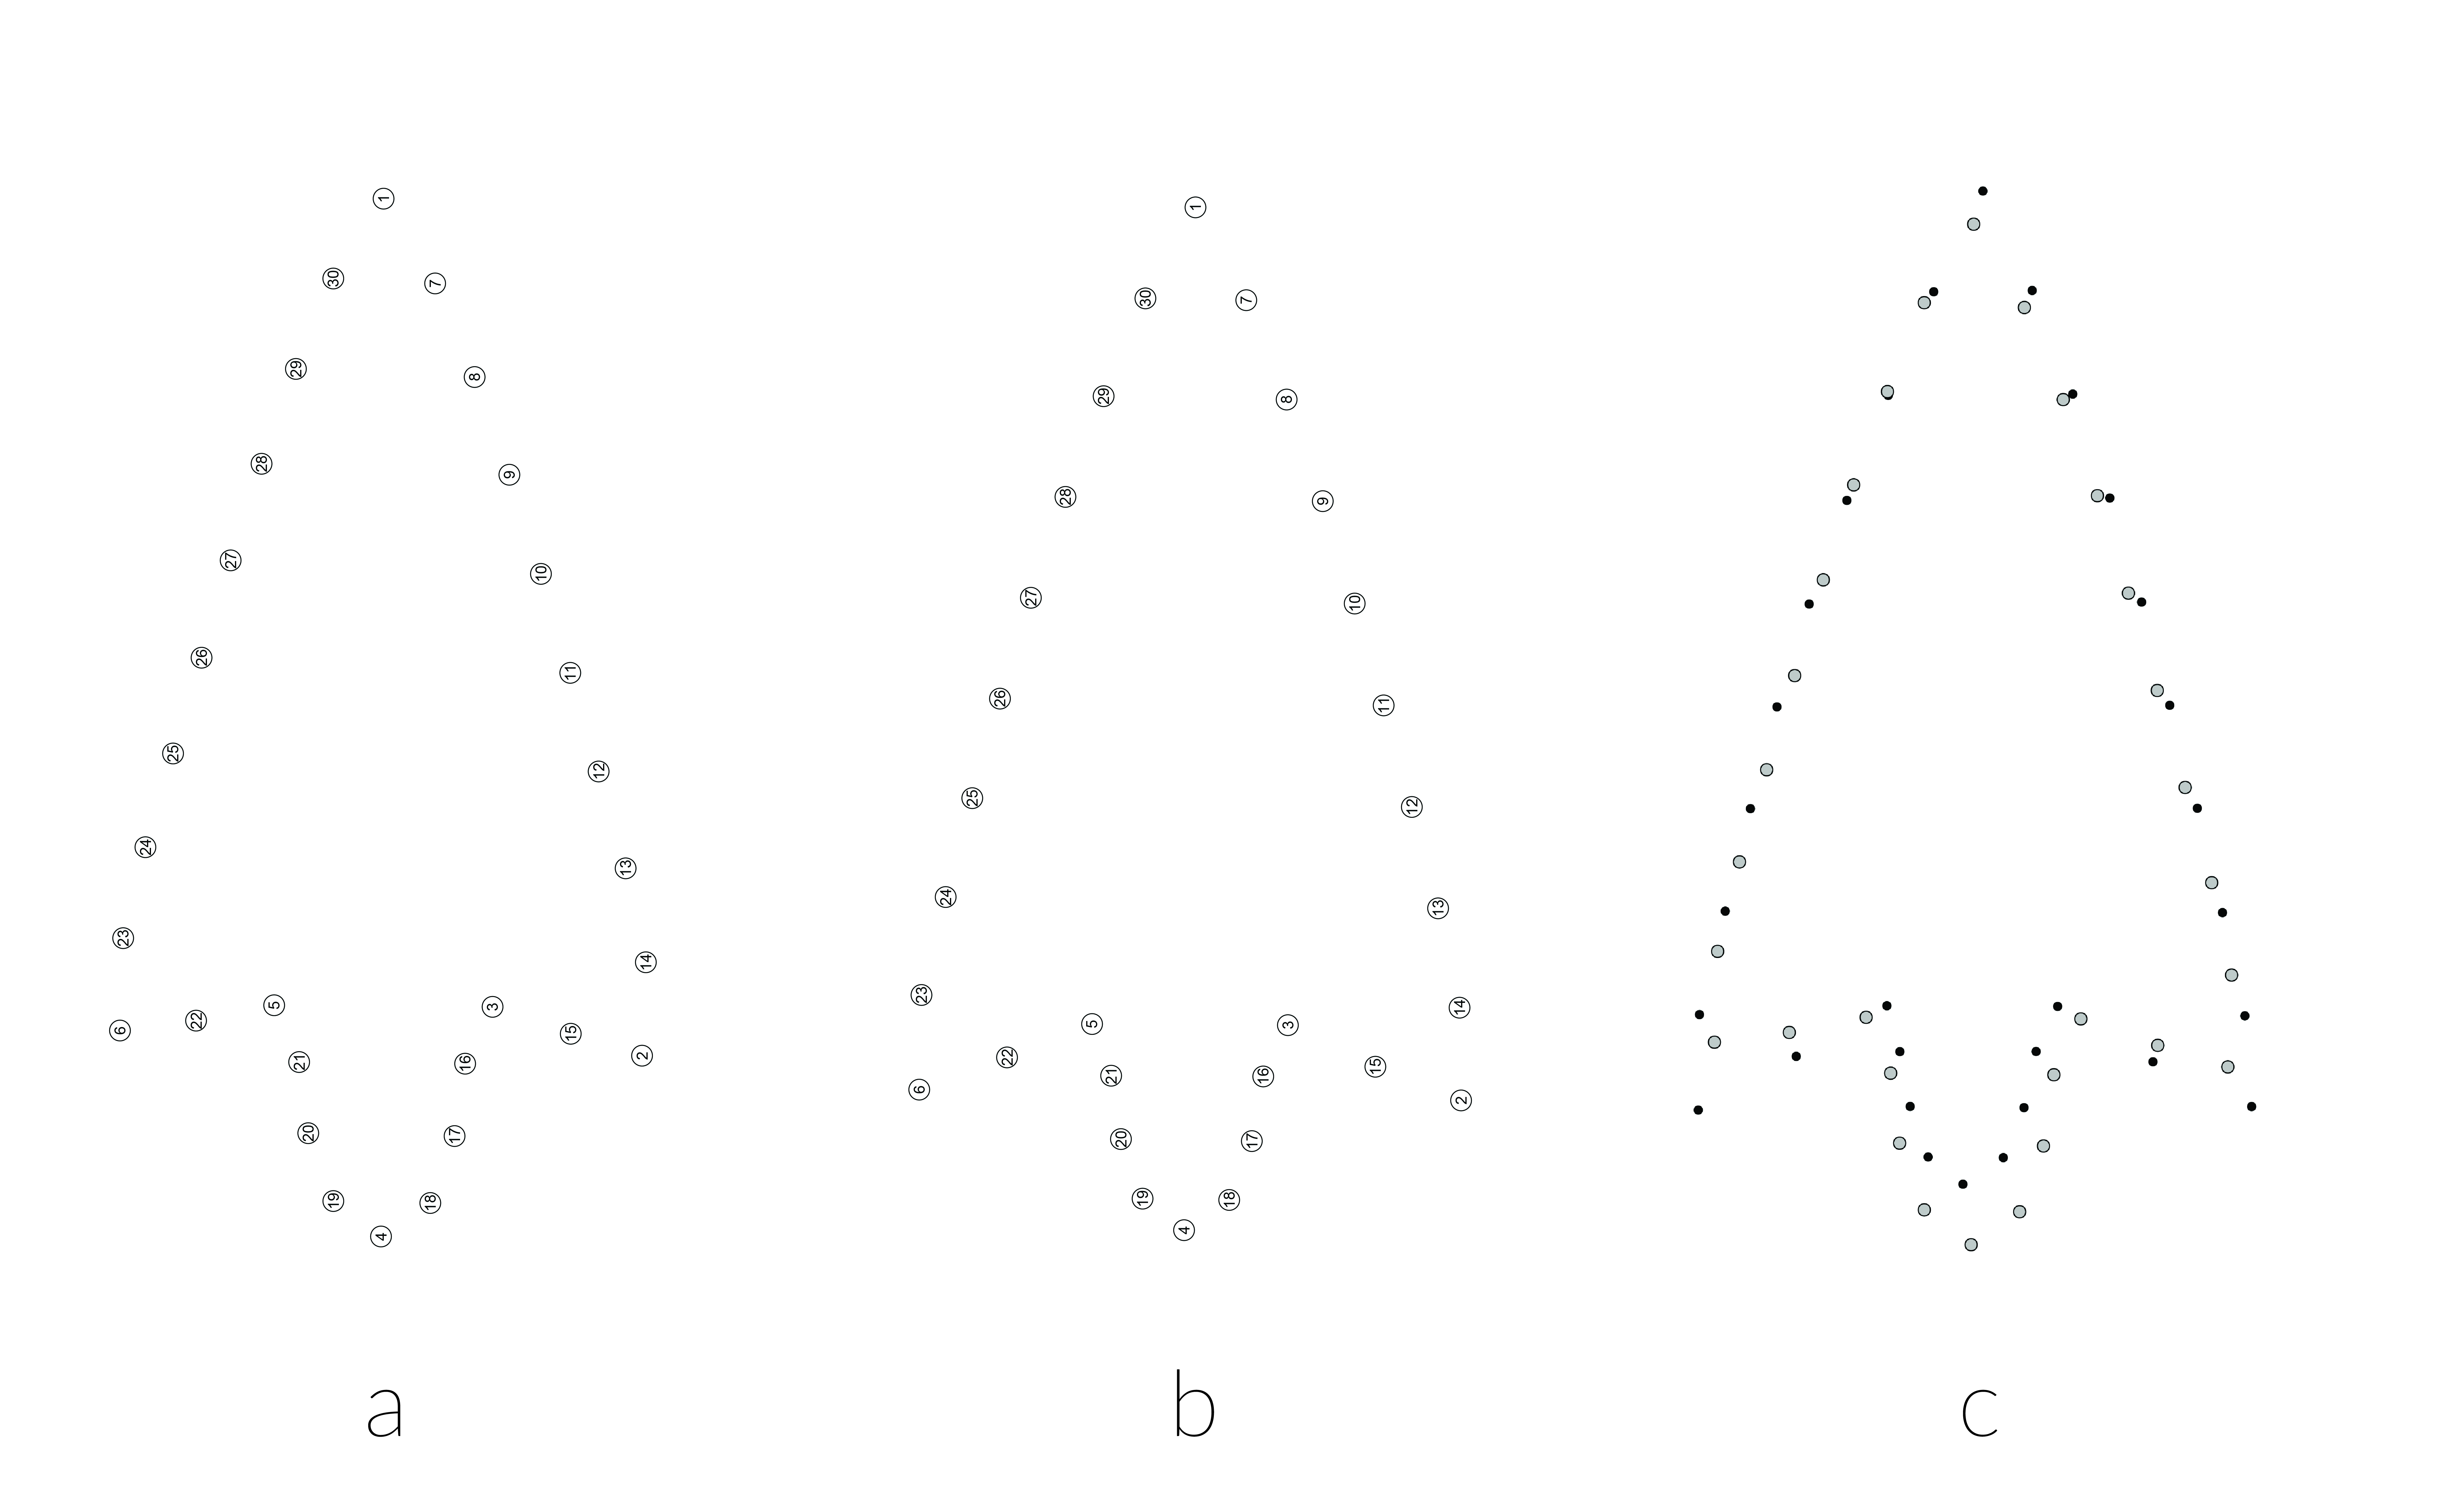
\includegraphics[width=1\linewidth]{ms-figs/figure5} \caption{Mean shapes for Perdiz arrow points from the northern (a, left), and southern (b, center) behavioral region. In the comparison of the two (c, right), the northern behavioral region is represented by gray circles, and the southern, by black. Additional information related to the mean shapes, including those data and code needed to reproduce these results, can be found in the supplemental materials at https://seldenlab.github.io/perdiz3/.}\label{fig:fig5}
\end{figure}

\hypertarget{discussion}{%
\section{Discussion}\label{discussion}}

The \emph{shape boundary} empirically delineates two discrete
\emph{behavioral regions} in the ancestral Caddo area. That the Perdiz
arrow points recovered from Caddo burials north and south of the
\emph{shape boundary} were found to differ significantly, expands the
scope of the \emph{behavioral regions} to include a third class of
artifacts (Caddo bottles, bifaces, and---now---arrow points) (Selden Jr,
et al.~2021; Selden Jr.~2018a, 2018b, 2019, 2021b; Selden Jr., et
al.~2020; Selden Jr., et al.~2018). This study clearly illustrates that
those morphological differences among Perdiz arrow points found in the
northern and southern \emph{behavioral regions} are predictable, and can
be identified using the standard suite of linear metrics regularly
collected as part of cultural resource management endeavors. The
geometric morphometric analysis demonstrated significant morphological
differences in basal morphology for Perdiz arrow points from the two
\emph{behavioral regions}.

\hypertarget{acknowledgments}{%
\section*{Acknowledgments}\label{acknowledgments}}
\addcontentsline{toc}{section}{Acknowledgments}

We express our gratitude to the Caddo Nation of Oklahoma and the
Anthropology and Archaeology Laboratory at Stephen F. Austin State
University for the requisite permissions and access to the NAGPRA
objects from the Washington Square Mound site and Turner collections,
and to Tom A. Middlebrook for brokering access to the Perdiz arrow
points from burials at the Morse Mound site. Thanks also to the editor
and reviewers for their useful comments and constructive criticisms,
which further improved this manuscript.

\hypertarget{data-management}{%
\section*{Data Management}\label{data-management}}
\addcontentsline{toc}{section}{Data Management}

The data and analysis code associated with this project can be accessed
through the GitHub repository
(\url{https://github.com/seldenlab/perdiz3}) or the supplementary
materials (\url{https://seldenlab.github.io/perdiz3/}); which are
digitally curated on the Open Science Framework at \newline DOI:
10.17605/OSF.IO/UK9ZD.


\bibliographystyle{spphys}
\bibliography{mybibfile.bib}

\end{document}
